\chapter{VALIDAÇÃO DO CÓDIGO NÚMERICO}
\label{validacao}
\section{\textbf{Introdução}}
Neste capítulo serão apresentados as comparações realizadas entre os resultados numéricos obtidos para x casos amplamente conhecidos na literatura e a solução analítica unidimensional dos mesmos.
Como a solução numérica é obtida para problemas bidimensionais, é preciso pegar uma seção transversal do domínio e interpolar  resultado, produzindo, assim, uma aproximação.
Dessa forma, a quantificação do erro relativo médio se faz necessária, com o objetivo de apresentar a acurácia do código numérico. O erro relativo entre a solução numérica e a solução analítica é calculado pela equação \eqref{error_eq}:
\begin{equation}
    er_i = \frac{|(val_a)_i - (val_n)_i|}{(val_a)_i}
    \label{error_eq} 
\end{equation}
onde $(val_a)_i$ é o valor encontrado pela solução analítica e $(val_n)_i$ é o valor encontrado pela solução numérica, ambos encontrados no nó $i$.

São calculados também a média e o desvio padrão dos erros relativos pelas equações \eqref{error_mean} e \eqref{error_mean}, respectivamente:
\begin{equation}
    er_{mean} = \frac{1}{N}\sum_{i=0}^{N} er_i
    \label{error_mean}
\end{equation}
\begin{equation}
    er_{std} = \left\| \frac{1}{N}\sum_{i=0}^{N} er_i-er_{mean} \right\|_2
    \label{error_std} 
\end{equation}

As validações foram organizadas em três seções que representam diferentes etapas da implementação do modelo matemático, sendo assim espera-se mostrar a aplicabilidade do código numérico desenvolvido, além do histórico de aprendizado obtido.
Na seção \ref{sec_solidos}, os problemas de transferência de calor em sólidos com condutividade termica constante são apresentados.
Os casos propostos nesta seção buscam confirmar a importação correta da malha e a montagem das matrizes globais, como também a aplicação das condições de contorno de Dirichlet e de Neumann.

Já na seção \ref{sec_fluidos}, os problemas com o termo convectivo presente são analisados.
Foi considerado o fluido como incompressível e newtoniano, dessa forma a equação de Navier-Stokes pode ser aplicada segundo a formulação corrente-vorticidade.
A estrutura do algoritmo de solução nos casos propostos dessa seção é a mesma utilizada na resolução do problema proposto neste trabalho.
Dessa forma, podemos confirmar a correta aplicação das condições de contorno da vorticidade que deve ser calculada em cada passo de tempo.
%No final da seção, apresentamos um caso onde o número de Reynolds é aumentado até as oscilações numéricas serem visualizadas e, assim, verificar o limite de aplicabilidade do código.

Finalmente, na seção \ref{sec_particulas}, é apresentado os clássicos casos de dinâmica em partículas com o intuito de validar as forças de gravidade, arrasto e sustentação isoladamente e, com isso, possibilitar uma a correção pontual no modelo quando
necessário, alem de permitir observar com maior precisão a influência da atuação que cada uma das força faz sobre a partícula.

Para casos com variáveis temporais, foi utilizado um critério de parada de $10^{-5}$ de variação de valores entre dois intervalos de tempo consecutivos.
Desta maneira espera-se que o sistema já tenha entrado na situação de convergência e esteja próximo o suficiente de seus valores finais.
Isto foi feito para poupar tempo de computação, para casos que possuem um limite de tempo elevado e convergem rapidamente, fazendo com que o código continuasse desnecessariamente.

A execução do código e a computação dos resultados foram realizados em um computador de uso pessoal com as seguintes especificações:
\begin{itemize}
    \item Dell Latitude E6410 com processador Intel® Core™ i5 CPU M 520 2.40GHz com 4 núcloes e 4Gb de memória RAM.
          O sistema operacional ubuntu 16.04 LTS e compilador Python 3.5.
\end{itemize}


%---------------------------------------------------------------------------------------------Validação de sólidos
\section{\textbf{Validações de Problemas em Sólidos}}
\label{sec_solidos}
%---------------------------------------------------------------------------------------------Primeiro Exemplo
\subsection{\textbf{Equação de Laplace com Condições de Contorno de Dirichlet}}
\label{sec_laplace_dir}
O problema de troca de calor em uma placa é um dos exemplos clássicos utilizados para estudar as equações de transmissão de calor em sólidos. O mais simples destes é uma barra unidimensional com condutividade térmica constante e sem geração de calor onde a temperatura é conhecida nas extremidades.
Como a malha do código foi desenvolvida para solução de problemas bidimensionais, cria-se um problema bidimensional com condições de contorno equivalentes e extrai-se uma seção para que se possa comparar os resultados.

Para a solução dos problemas em sólidos e fluidos no espaço foi utilizado o Método de Elementos Finitos, apresentado na seção \ref{mef}.
Enquanto para a aproximação da dinâmica das partículas e solução dos sólidos e fluidos no tempo utilizou-se o Método de Diferenças Finitas, explicado na seção \ref{mdf}.

A equação de governo deste fenômeno é conhecida como a equação de Laplace \eqref{laplace_d_perm_eq} para sólidos em estado permanente e é apresentada a seguir:
\begin{equation}
    \nabla^2 T = 0
    \label{laplace_d_perm_eq} 
\end{equation}
onde T é a temperatura na placa e $\nabla^2$ é o operador diferencial conhecido como laplaciano.

E a solução analítica do problema unidimensional associado é:
\begin{equation}
    T(x) = \dfrac{T_L-T_0}{L} x + T_0
    \label{laplace_d_sol}
\end{equation}
onde $L$ é o comprimento da barra, $T_0$ e $T_L$ são, respectivamente, os valores da temperatura em $x=0$ e $x=L$.

As condições de contorno e o dominio bidimensional utilizados na simulação são apresentados na \ref{laplace_d_bc}. A condição de fluxo de calor $\dfrac{\partial T}{\partial n}$ nulo significa que nenhuma condição é imposta no contorno.

\begin{figure}[H]
    \centering
    \stackunder{
        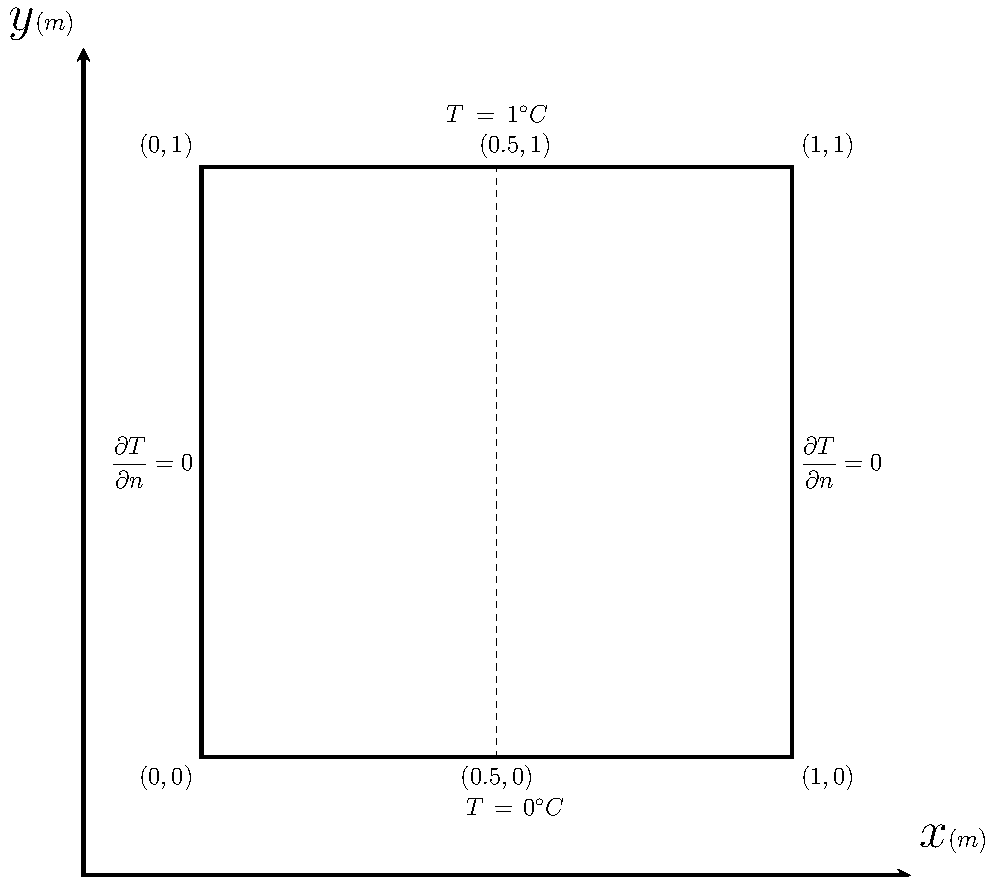
\includegraphics[width=.7\linewidth]{figures/laplace_dirichlet_boundary_conditions.pdf}
    } {\raggedleft \scriptsize Fonte: Autor.}
    \caption{Condições de contorno da placa para o problema de Laplace \ref{sec_laplace_dir}.}
    \label{laplace_d_bc}
\end{figure}

O dominio foi discretizado utilizando uma malha triangular linear não estruturada com 3162 elementos e 568 nós.
A malha foi criada pelo o software GMSH como proposto por Geuzaine e Remacle (2009)\cite{gmsh} e importada ao código numérico.
A \ref{laplace_d_3d} apresenta o campo de temperatura, onde os eixos $x$ e $y$ representam o dominio e o eixo $z$ é a distribuição de temperatura, e que é possível observar que o campo de temperatura possui um perfil linear variando de 0 (cor azul) a 1 (cor vermelha).
\begin{figure}[H]
    \centering
    \stackunder{
        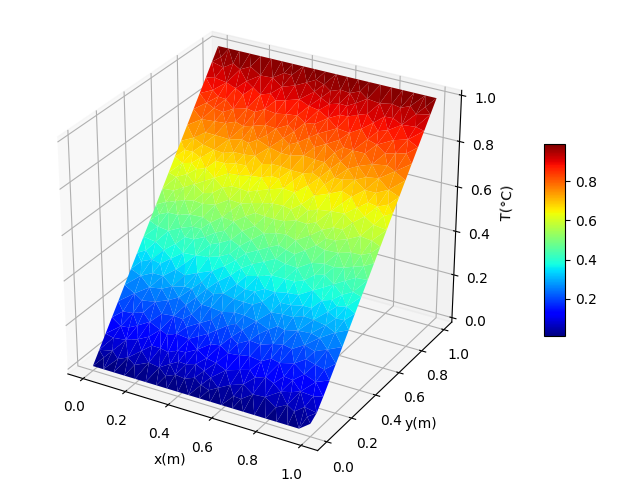
\includegraphics[width=.7\linewidth]{figures/laplace_dirichlet_permanent_3d.png}
    } {\raggedleft \scriptsize Fonte: Autor.}
    \caption{Distribuição de temperaturas na placa da solução permanente da equação de Laplace \ref{sec_laplace_dir}.}
    \label{laplace_d_3d}
\end{figure}

A comparação entre os resultados da solução analítica \eqref{laplace_d_sol} e a solução numerica, para a seção $x=0.5m$, é apresentada na \ref{laplace_d_perm_comp}, onde é possível observar que ambas possuem o mesmo perfil.
Essa proximidade é quantificada pelo erro relativo médio que foi de $0.08929\%$ e com desvio padrão de $0.06698\%$
\begin{figure}[H]
    \centering
    \stackunder{
        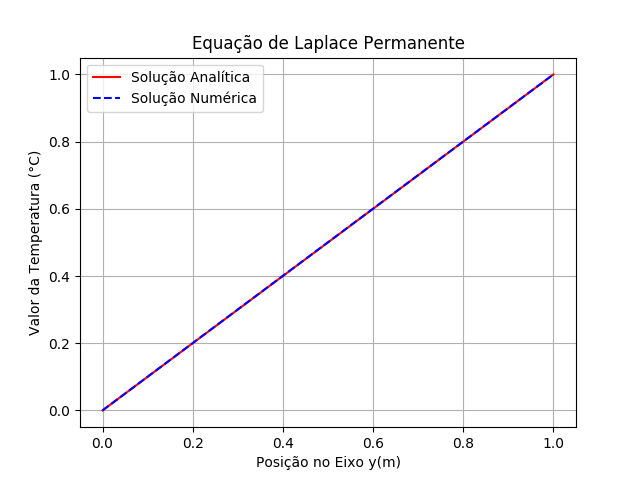
\includegraphics[width=.7\linewidth]{figures/laplace_dirichlet_permanent_comparison.png}
    } {\raggedleft \scriptsize Fonte: Autor.}
    \caption{Comparação de resultado das solução númerica e analítica do caso de transporte de temperatura em sólidos no regime permanente.}
    \label{laplace_d_perm_comp}
\end{figure}

Ao solucionar o mesmo problema introduzindo o termo transiente na equação de governo \ref{laplace_d_perm_eq}, pode-se verificar a evolução de comportamento da temperatura ao longo do tempo.
Dessa forma, a equação que representa este caso é:
\begin{equation}
    \dfrac{\partial T}{\partial t} + k\nabla^2 T = 0
    \label{laplace_d_trans_eq} 
\end{equation}
onde $k$ é o coeficiente de condutividade térmica da placa e $t$ é a variável temporal.

Porém, ao longo dos passos de tempo, a solução se aproxima de um problema permanente, portanto pode-se fazer a comparação dos resultados obtidos neste exemplo com os valores da solução analítica \eqref{laplace_d_sol}, tomando-se que $t\rightarrow \infty$.
As condições iniciais $t=0s$ atribuídas aos nós sem condição de contorno foram de um valor inicial de $0^{\circ}C$.
A \ref{laplace_d_trans_comp} apresenta a evolução do campo de temperaturas em função do tempo.
É possível observar que a solução numérica converge para a solução analítica formando um perfil linear.
O erro relativo médio calculado para este caso foi de $0.08276\%$ e com desvio padrão de $0.06340\%$.
\begin{figure}[H]
    \centering
    \stackunder{
        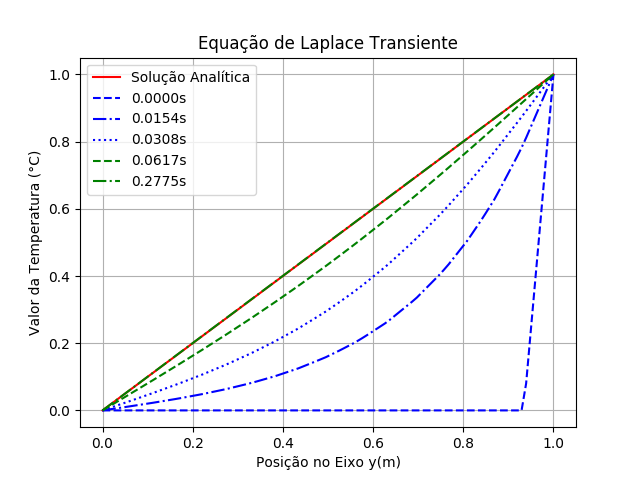
\includegraphics[width=.7\linewidth]{figures/laplace_dirichlet_transient_comparison.png}
    } {\raggedleft \scriptsize Fonte: Autor.}
    \caption{Comparação de resultado das soluções númericas e analítica de transporte em sólidos no regime transiente.}
    \label{laplace_d_trans_comp}
\end{figure}


%---------------------------------------------------------------------------------------------Segundo Exemplo
\subsection{\textbf{Equação de Poisson com Condições de Contorno de Dirichlet}}
\label{sec_poisson_dir}
Neste problema busca-se estudar o comportamento de uma placa com geração de calor em seu domínio e temperaturas fixas nas laterais.
Novamente, para permitir a comparação de resultados, é extraída uma seção da placa para observar os resultados como um problema unidimensional.

A equação que governa este caso é denomidada equação de Poisson \eqref{poisson_d_perm_eq}, tomada para um problema permanente, ou seja sem variação no tempo.
\begin{equation}
    -k\nabla^2 T = Q
    \label{poisson_d_perm_eq} 
\end{equation}
onde $Q$ é a geração de calor na placa.

A solução analítica para o caso de uma barra unidimensional é apresentada embaixo:
\begin{equation}
    T(x) = \dfrac{Q}{2k}\left(-x^2 + L x\right) + \dfrac{T_L-T_0}{L} x + T_0
    \label{poisson_d_sol} 
\end{equation}

As condições de contorno e o dominio bidimensional utilizados na simulação são apresentados na \ref{poisson_d_bc}.
A geração de calor utilizada foi de $Q = 40W/m^3$ e a condutividade termica foi de $k=5 W/m^{\circ}C$.
\begin{figure}[H]
    \centering
    \stackunder{
        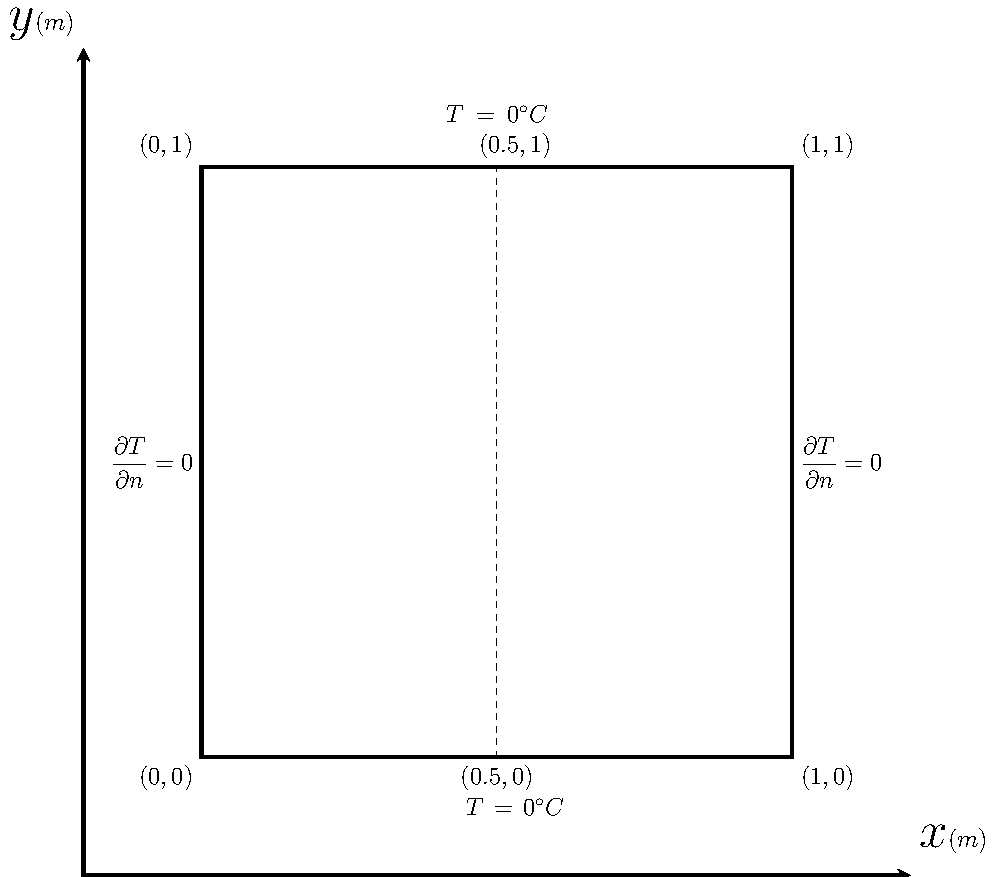
\includegraphics[width=.7\linewidth]{figures/poisson_dirichlet_boundary_conditions.pdf}
    } {\raggedleft \scriptsize Fonte: Autor.}
    \caption{Condições de contorno da placa para o problema de Poisson \ref{sec_poisson_dir}.}
    \label{poisson_d_bc}
\end{figure}

Novamente, foi utilizada uma malha triangular linear não estruturada com 3162 elementos e 568 nós.
A \ref{poisson_d_3d} apresenta o campo de temperatura, onde os eixos $x$ e $y$ representam o dominio e o eixo $z$ é a distribuição de temperatura, onde é possível observar que o campo de temperatura possui um perfil parabólico variando de 0 (cor azul) a 1 (cor vermelha).
\begin{figure}[H]
    \centering
    \stackunder{
        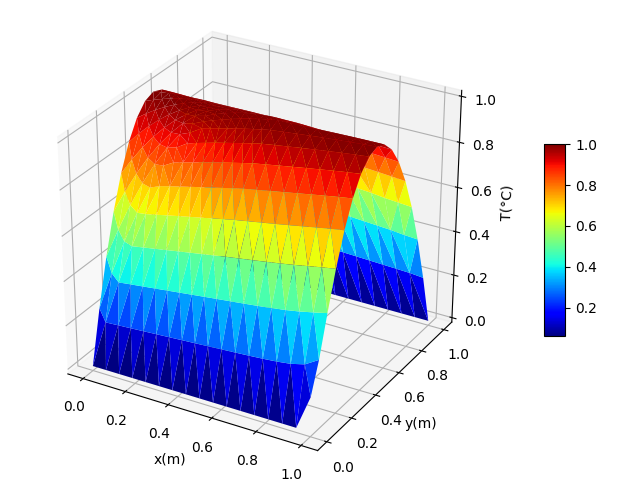
\includegraphics[width=.7\linewidth]{figures/poisson_dirichlet_permanent_3d.png}
    } {\raggedleft \scriptsize Fonte: Autor.}
    \caption{Distribuição de temperaturas na placa da solução do problema permanente de Poisson \ref{sec_poisson_dir}.}
    \label{poisson_d_3d}
\end{figure}

A comparação entre os resultados da solução analítica \eqref{poisson_d_sol} e a solução numerica, para a seção $x=0.5m$, é apresentada na \ref{poisson_d_perm_comp}, onde é possível observar que ambas possuem o mesmo perfil.
Essa proximidade é quantificada pelo erro relativo médio que foi de $0.21048\%$ e com desvio padrão de $0.40921\%$.
\begin{figure}[H]
    \centering
    \stackunder{
        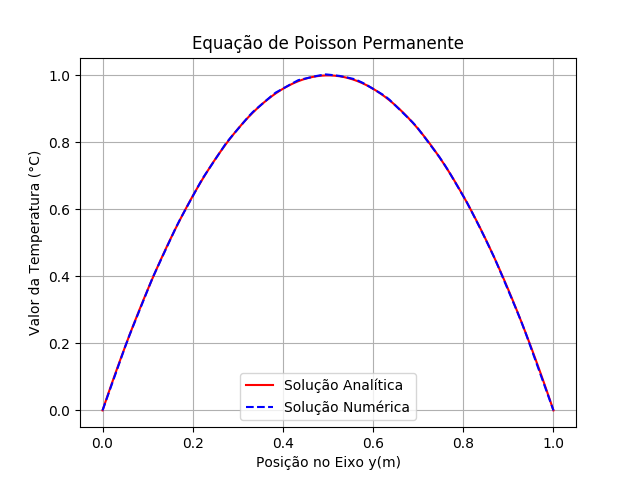
\includegraphics[width=.7\linewidth]{figures/poisson_dirichlet_permanent_comparison.png}
    } {\raggedleft \scriptsize Fonte: Autor.}
    \caption{Comparação de resultado das solução númerica e analítica do problema de transporte de temperatura em sólidos no regime permanente com geração de calor.}
    \label{poisson_d_perm_comp}
\end{figure}

A seguir, é apresentado o resultado com termo transiente $\dfrac{\partial T}{\partial t}$ tendendo a um estado permanente.
As condições iniciais $t=0s$ atribuídas aos nós sem condição de contorno foram de um valor inicial de $0^{\circ}C$.
A \ref{poisson_d_trans_comp} apresenta a evolução do campo de temperaturas em função do tempo.
É possível observar que a solução numérica converge para a solução analítica formando um perfil parabólico.
O erro relativo médio calculado para este caso foi de $0.21101\%$ e com desvio padrão de $0.40994\%$.
\begin{figure}[H]
    \centering
    \stackunder{
        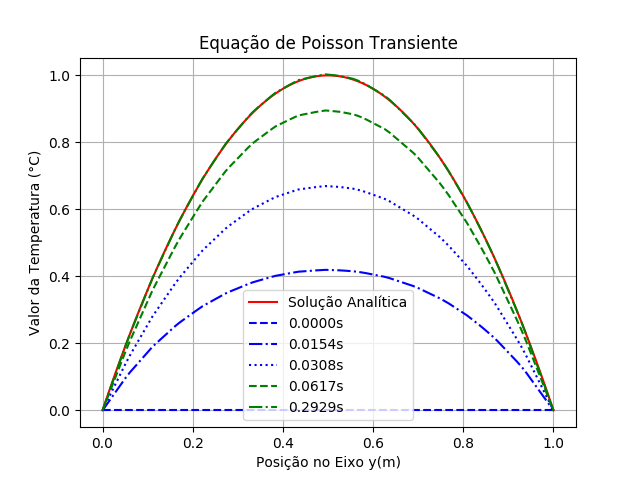
\includegraphics[width=.7\linewidth]{figures/poisson_dirichlet_transient_comparison.png}
    } {\raggedleft \scriptsize Fonte: Autor.}
    \caption{Comparação de resultado das soluções númericas e analítica do problema de trasnporte de temperatura em sólidos no regime transiente com geração de calor.}
    \label{poisson_d_trans_comp}
\end{figure}

%---------------------------------------------------------------------------------------------Terceiro Exemplo
\subsection{\textbf{Equação de Poisson com Condições de Contorno de Dirichlet e Neumann}}
\label{sec_poisson_neu}
Este caso foi escolhido para validar a solução de problemas com condições de contorno de Neumann.
Trata-se de uma placa com temperatura fixa em uma das paredes e no lado oposto é defido um valor para o fluxo de calor presente.
Toma-se uma seção da placa para observar os resultados e compará-los com um problema unidimensional de uma barra com as mesmas condições presentes.

A equação de governo é novamente a equação de Poisson \eqref{poisson_d_perm_eq}, e sua solução analítica para uma barra unidimensional é dada por:
\begin{equation}
    T(x) = \dfrac{Q}{k}\left(\dfrac{-x^2}{2} + L x\right) - \dfrac{q}{k} x + T_0
    \label{poisson_n_sol} 
\end{equation}
onde $q$ é o fluxo de calor na extremidade $x=L$.

As condições de contorno e o dominio bidimensional utilizados na simulação são apresentados na \ref{poisson_n_bc}.
A geração de calor utilizada foi de $Q = -7W/m^3$, a condutividade termica foi de $k=5 W/m^{\circ}C$ e o fluxo de calor foi de $q = -5 W/m^2$.
\begin{figure}[H]
    \centering
    \stackunder{
        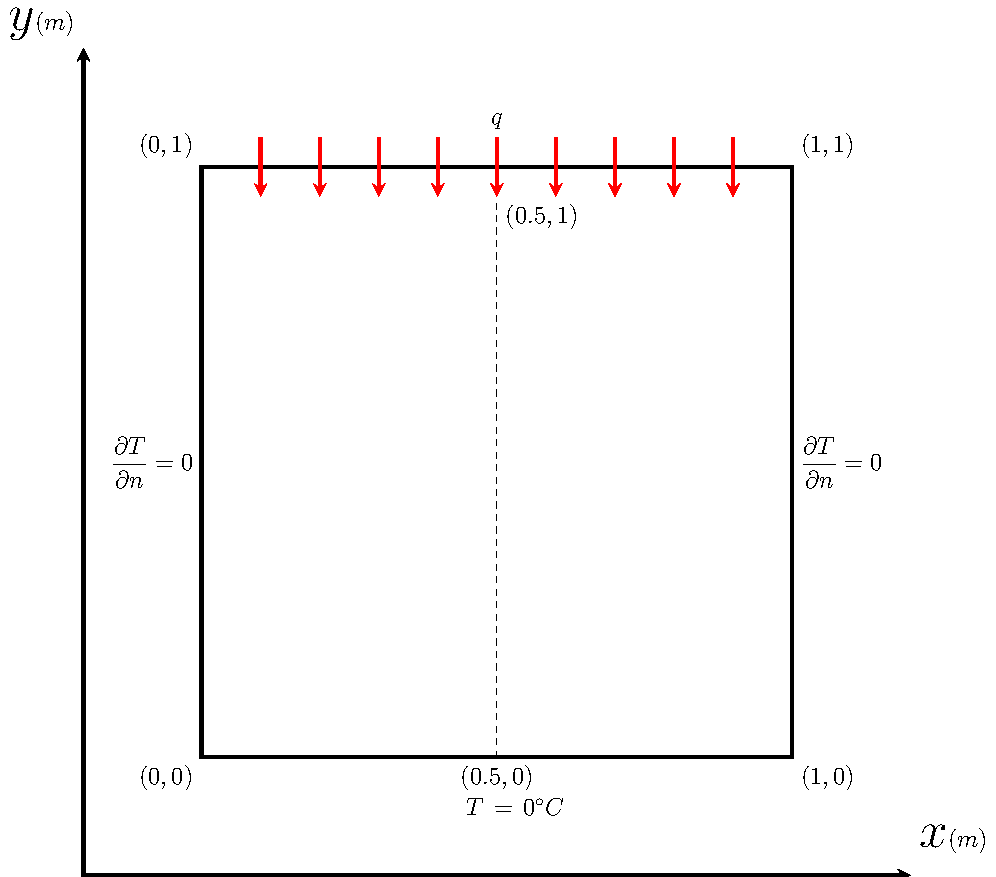
\includegraphics[width=.7\linewidth]{figures/poisson_neumann_boundary_conditions.pdf}
    } {\raggedleft \scriptsize Fonte: Autor.}
    \caption{Condições de contorno da placa para o problema de Poisson \ref{sec_poisson_neu}.}
    \label{poisson_n_bc}
\end{figure}

Novamente, foi utilizada uma malha triangular linear não estruturada com 3162 elementos e 568 nós.
A \ref{poisson_n_3d} apresenta o campo de temperatura, onde os eixos $x$ e $y$ representam o dominio e o eixo $z$ é a distribuição de temperatura variando de 0 (cor azul) a 0.35 (vermelha).
\begin{figure}[H]
    \centering
    \stackunder{
        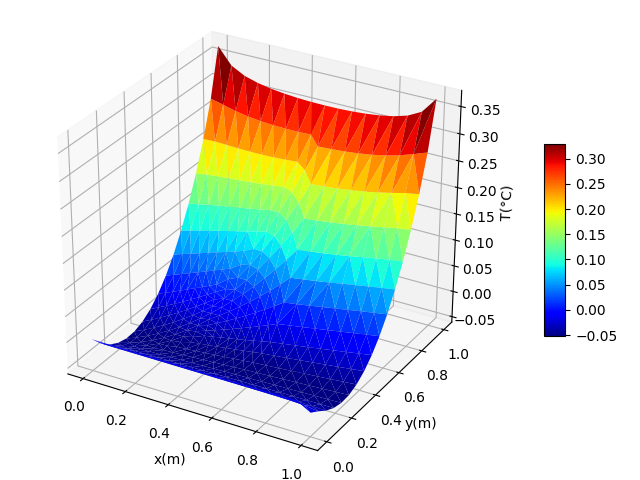
\includegraphics[width=.7\linewidth]{figures/poisson_neumann_permanent_3d.png}
    } {\raggedleft \scriptsize Fonte: Autor.}
    \caption{Distribuição de temperaturas na placa da solução do problema permanente de Poisson \ref{sec_poisson_neu}.}
    \label{poisson_n_3d}
\end{figure}

A comparação entre os resultados da solução analítica \eqref{poisson_n_sol} e a solução numérica, para a seção $x=0.5m$, é apresentada na \ref{poisson_n_perm_comp}, onde pode-se observar que ambas possuem o mesmo perfil.
A semelhança entre elas é quantificada pelo erro relativo médio que foi de $0.427\%$ e com desvio padrão de $0.8414\%$:
\begin{figure}[H]
    \centering
    \stackunder{
        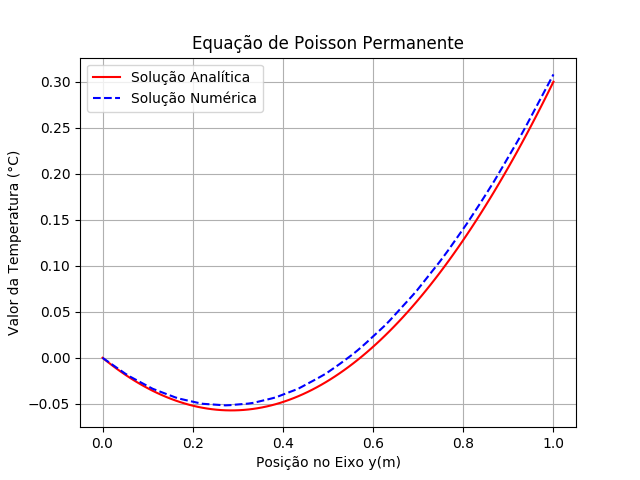
\includegraphics[width=.7\linewidth]{figures/poisson_neumann_permanent_comparison.png}
    } {\raggedleft \scriptsize Fonte: Autor.}
    \caption{Comparação de resultado das solução númerica e analítica do problema de transporte de temperatura em sólidos no regime permanente com geração e fluxo de calor.}
    \label{poisson_n_perm_comp}
\end{figure}

As condições iniciais $t=0s$ atribuídas aos nós sem condição de contorno foram de um valor inicial de $0^{\circ}C$.
A \ref{poisson_n_trans_comp} apresenta a evolução do campo de temperaturas em função do tempo.
É possível observar que a solução numérica converge para a solução analítica.
O erro relativo médio calculado para este caso foi de $0.31\%$ e com desvio padrão de $0.9205\%$.
\begin{figure}[H]
    \centering
    \stackunder{
        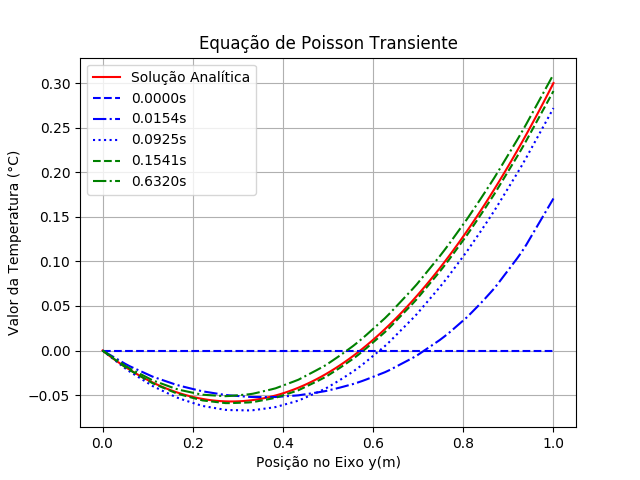
\includegraphics[width=.7\linewidth]{figures/poisson_neumann_transient_comparison.png}
    } {\raggedleft \scriptsize Fonte: Autor.}
    \caption{Comparação de resultado das soluções númericas e analítica do problema de transporte de temperatura em sólidos no regime permanente com geração e fluxo de calor.}
    \label{poisson_n_trans_comp}
\end{figure}

%---------------------------------------------------------------------------------------------Validação de fluidos
\section{\textbf{Validações de Problemas em Fluídos}}
\label{sec_fluidos}
%---------------------------------------------------------------------------------------------Primeiro Exemplo
\subsection{\textbf{Escoamento de Poiseuille}}
\label{sec_poiseuille}
Como indicado anteriormente, foi utilizado o Método de Elementos Finitos para a solução do campo de velocidades no espaço, e o Método de Diferenças Finitas no tempo.

Este é um dos primeiros exemplos dados ao estudar-se a meĉanica dos fluidos e a equação de Navier-Stoakes\eqref{navier}, pois trata-se de uma configuração geométrica muito simples.
O escoamento de Poiseuille também é conhecido como escoamento entre placas paralelas, já que essa é exatamente a descrição de sua forma e as placas são tomadas como estacionárias em relação ao fluido.

O escoamento ocorre entre duas placas paralelas de comprimento infinito com uma distância constante entre elas.
É tomado um fluído ideal, isto é, newtoniano, imcompressível e em estado permanente com seu perfil plenamente desenvolvido.
As condições de contorno são definidas para a função corrente e a velocidade.
Para os valores iniciais nos nós sem condição de contorno foram arbitrados como nulos.

Como apresentado por Pontes e Norberto (2010)\cite{pontes_norberto}, o sistema de equações de governo deste escoamento é o sistema corrente-vorticidade \ref{corrente_vorticidade}, e a solução analítica do perfil de velocidades é dada por:
\begin{equation}
    v_x(y) = \dfrac{4U_{max}}{L^2}y(L-y)
    \label{poiseuille_sol} 
\end{equation}
onde $v_x$ é velocidade do fluido na direção do eixo $x$, $L$ é o comprimento das placas e $U_{max}$ é a velocidade máxima do escoamento.

Para esta simulação foram usadas as condições de contorno e o dominio bidimensional apresentados na \ref{poiseuille_bc}.
A velocidade máxima $U_{max}$ é tomada em função da velocidade de entrada $U$ na relação $U_{max}=1.5U$.
Foi escolhido um valor para o número de Reynolds\eqref{reynolds} de $Re=1$ e um intervalo de tempo $dt=0.1s$.
\begin{figure}[H]
    \centering
    \stackunder{
        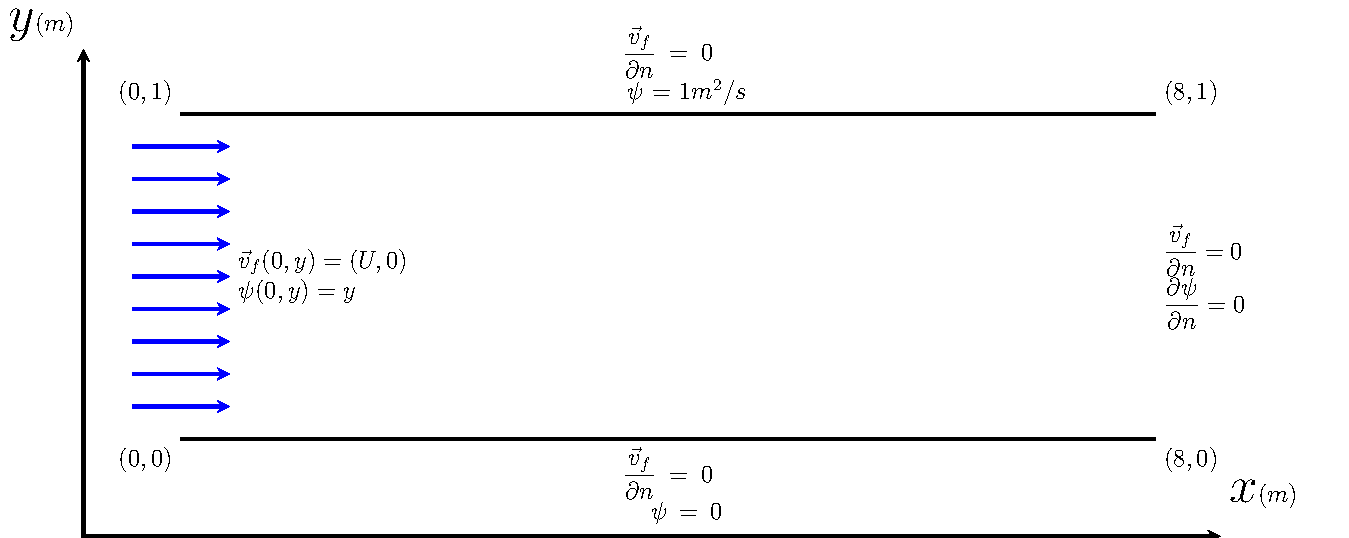
\includegraphics[width=\linewidth]{figures/Poiseuille_boundary_conditions.pdf}
    } {\raggedleft \scriptsize Fonte: Autor.}
    \caption{Condições de contorno de um escoamento entre placas paralelas de Poiseuille \ref{sec_poiseuille}.}
    \label{poiseuille_bc}
\end{figure}

A \ref{poiseuille_comp} apresenta a evolução do perfil de velocidades de uma seção tomada em $x=0.75L=6.0m$ em função do tempo.
Foi utilizada uma malha triangular linear não estruturada com 4200 elementos e 781 nós.
Nota-se que a solução numérica converge para a solução analítica ao se aproximar do estado permanente.
O erro relativo médio calculado para este caso foi de $4.587\%$ e com desvio padrão de $5.3501\%$.
\begin{figure}[H]
    \centering
    \stackunder{
        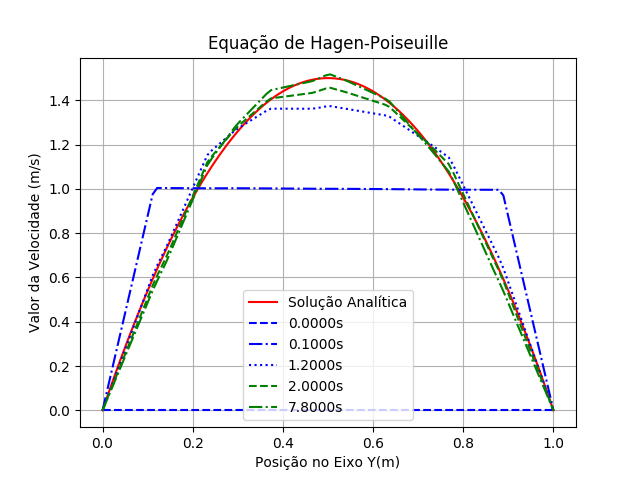
\includegraphics[width=.7\linewidth]{figures/Poiseuille_validation.png}
    } {\raggedleft \scriptsize Fonte: Autor.}
    \caption{Comparação de resultado das soluções númericas e analítica \ref{poiseuille_sol} do problema de corrente-vorticidade no regime permanente.}
    \label{poiseuille_comp}
\end{figure}

%---------------------------------------------------------------------------------------------Segundo Exemplo
\subsection{\textbf{Escoamento de Couette}}
\label{sec_couette}
Similar ao escoamento de Poiseuille\ref{sec_poiseuille}, entre duas placas paralelas de comprimento infinito separadas por uma distância constante.
Porém, neste caso, as placas possuem uma velocidade relativa entre si, ou seja, estão em movimento.
Novamente, utiliza-se a aproximação do escoamento para um fluído newtoniano, imcompressível e em estado permanente com seu perfil plenamente desenvolvido.
As condições de contorno são definidas para a função corrente e a velocidade, com os valores iniciais nos nós sem condição de contorno arbitrados como nulos.

Novamente trabalha-se com o sistema corrente-vorticidade \ref{corrente_vorticidade} e a solução analítica do perfil de velocidades é apresentada por Pontes e Norberto (2010)\cite{pontes_norberto}:
\begin{equation}
    v_x(y) = \dfrac{U_{sup} - U_{inf}}{L}y + U_{inf}
    \label{couette_sol} 
\end{equation}
onde $U_{sup}$ e $U_{inf}$ são as velocidades das placas superior e inferior, respectivamente.

Para esta simulação foram usadas as condições de contorno e o dominio bidimensional apresentados na \ref{couette_bc}.
Foram tomadas as velocidade superior como $U_{sup}=1m/s$ e $U_{inf}=-1m/s$ para um escoamente com número de Reynolds de $Re=1$ e um intervalo de tempo $dt=1.0s$.
\begin{figure}[H]
    \centering
    \stackunder{
        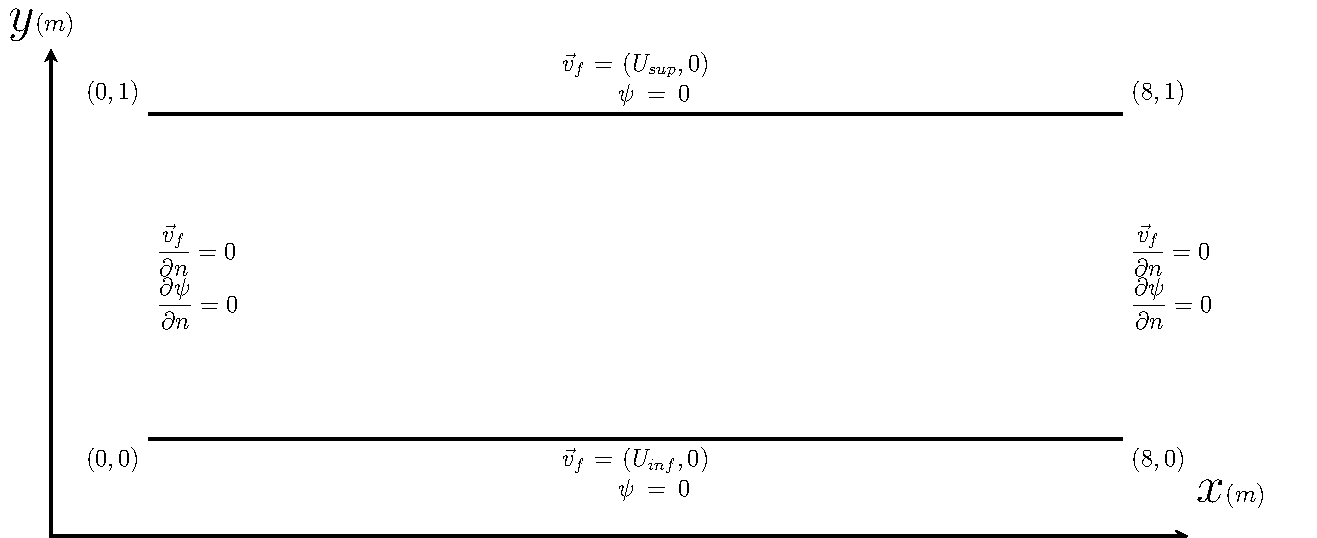
\includegraphics[width=\linewidth]{figures/Couette_boundary_conditions.pdf}
    } {\raggedleft \scriptsize Fonte: Autor.}
    \caption{Condições de contorno de um escoamento entre placas paralelas de Couette \ref{sec_couette}.}
    \label{couette_bc}
\end{figure}

A \ref{couette_comp} apresenta a evolução do perfil de velocidades de uma seção tomada em $x=0.5L=4.0m$ em função do tempo.
Novamente utilizou-se uma malha triangular linear não estruturada com 4200 elementos e 781 nós.
Pode-se observar que a solução numérica converge para a solução analítica ao se aproximar do estado permanente.
O erro relativo médio calculado para este caso foi de $1.4251\%$ e com desvio padrão de $27.934\%$.
\begin{figure}[H]
    \centering
    \stackunder{
        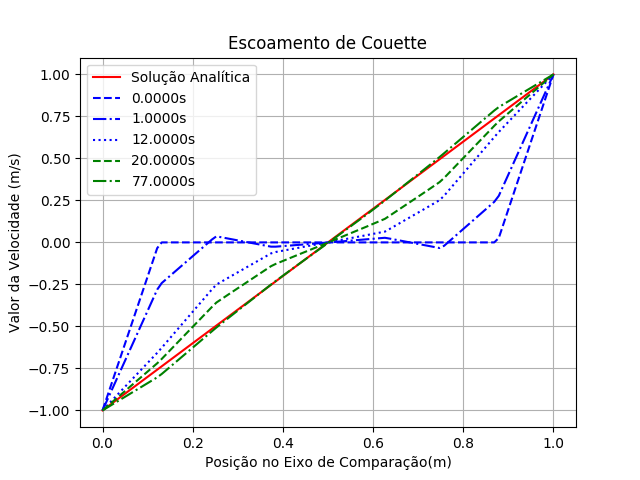
\includegraphics[width=.7\linewidth]{figures/Couette_validation.png}
    } {\raggedleft \scriptsize Fonte: Autor.}
    \caption{Comparação de resultado das soluções númericas e analítica \ref{couette_sol} do problema de corrente-vorticidade no regime permanente.}
    \label{couette_comp}
\end{figure}

%---------------------------------------------------------------------------------------------Terceiro Exemplo
% \subsection{\textbf{Escoamento de Cavidade (\textit{Lid-Driven Cavity Flow})}}


%---------------------------------------------------------------------------------------------Validação de partículas
\section{\textbf{Validações de Problemas em Partículas}}
\label{sec_particulas}
A simulação das forças é realizada sobre uma partícula isolada inserida em um malha com um escoamento com campo de velocidades constante em função da posição da partícula no eixo $y$, para facilitar os cálculos das soluções analíticas.
O campo de velocidades é arbitrado e não calculado como anteriormente.

Conforme indicado, foi utilizado o Método de Diferenças Finitas para discretização e solução da dinâmica das partículas.

Na \ref{force_bc}, é apresentado o domínio utilizado para os casos de validação das forças que atuam sobre a partícula, como também o campo de velocidade do fluido e a velocidade da partícula, além da sua posição inicial.
Para o caso da força de sustentação, foi necessário a utilização de um outro campo de velocidade conforme será apresentado mais a frente.
Enquanto que para o caso da força virtual, foi necessário assumir que o campo de velocidade do fluido dependesse da variável temporal.
O domínio foi discretizado utilizando uma malha triangular linear não estruturada com 2304 elementos e 417 nós.
\begin{figure}[H]
    \centering
    \stackunder{
        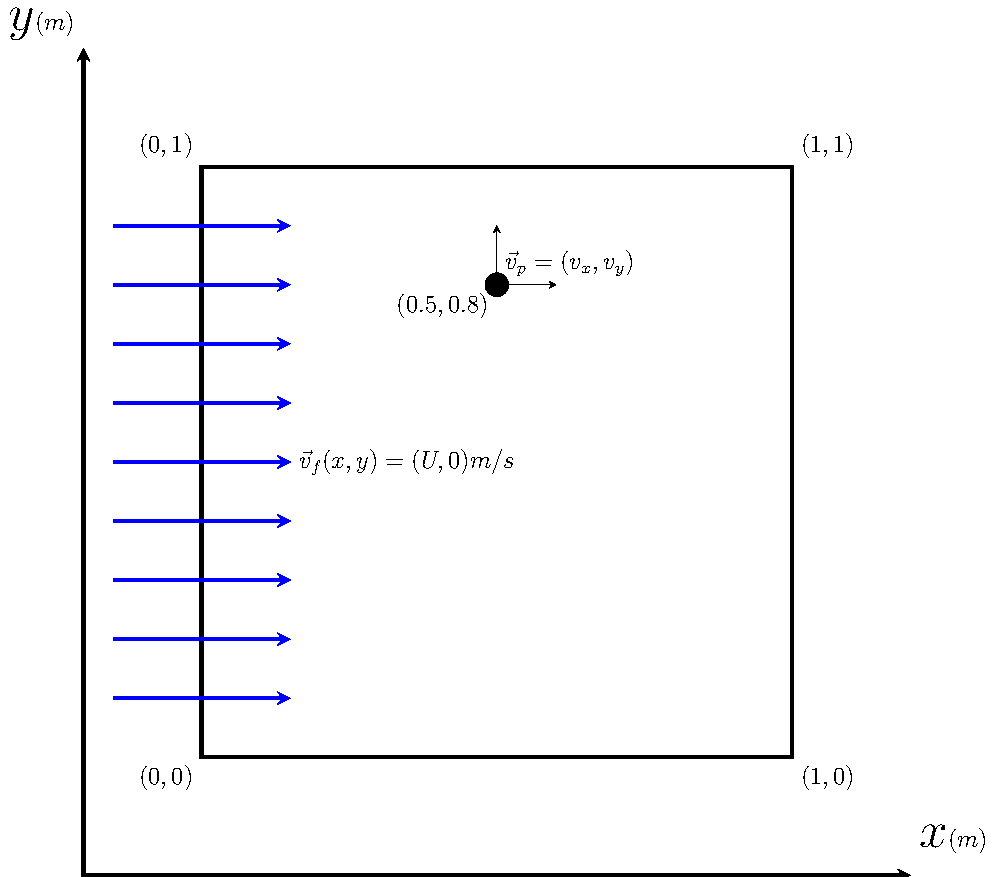
\includegraphics[width=0.7\linewidth]{figures/forces_boundary_conditions.pdf}
    } {\raggedleft \scriptsize Fonte: Autor.}
    \caption{Condições de contorno de uma partícula isolada sob efeito de uma força.}
    \label{force_bc}
\end{figure}

A validação das forças é feita individualmente, para que se possa comparar os valores do movimento simulado da partícula com a curva da solução analítica esperada.
Os parâmetros definidos para as simulações foram: uma partícula com diâmetro $d_p=0.001m$, densidade $\rho_p=30000Kg/m^3$, variação de tempo $dt=1.5625e^{-6}s$, tempo total $t_{max}=0.4s$, em um fluido com densidade $\rho_p=1000Kg/m^3$ e viscosidade dinâmica $0.89e^{-3}Pa.s$.

%---------------------------------------------------------------------------------------------Primeiro Exemplo
\subsection{\textbf{Força Gravitacional}}
\label{sec_grav}
A força gravitacional é a primeira e mais simples implementação de uma força.
A partícula é acelerada pela constante de aceleração gravitacional.
A validação deste caso permite verificar a base da estrutura de movimentação de partículas do código.

Para o caso de uma partícula isolada sob efeito da força gravitacional, a solução analítica para a posição da partícula no eixo $y$ é:
\begin{equation}
    y(t) = -\dfrac{g}{2}t^2 + v_{y0}t + p_{y0}
    \label{grav_sol} 
\end{equation}
onde $g$ é a aceleração da gravidade, tomada como $g=9.80665m/s^2$, $v_{y0}$ é a velocidade e $p_{y0}$ a posição inicial da partícula no eixo $y$.

Para a força gravitacional, utilizou-se uma malha com as condições e posição inicial apresentadas na \ref{force_bc}.
A velocidade inicial tomada foi $v_{y0}=0$.
Na \ref{grav_comp} pode-se observar a evolução da posição da partícula no eixo $y$ em função do tempo.
Foi utilizado um campo de velocidades com valor constante de $U=2m/s$.
O erro relativo médio calculado para este caso foi de $7.706e^{-4}\%$ e com desvio padrão de $1.753e^{-3}\%$.
\begin{figure}[H]
    \centering
    \stackunder{
        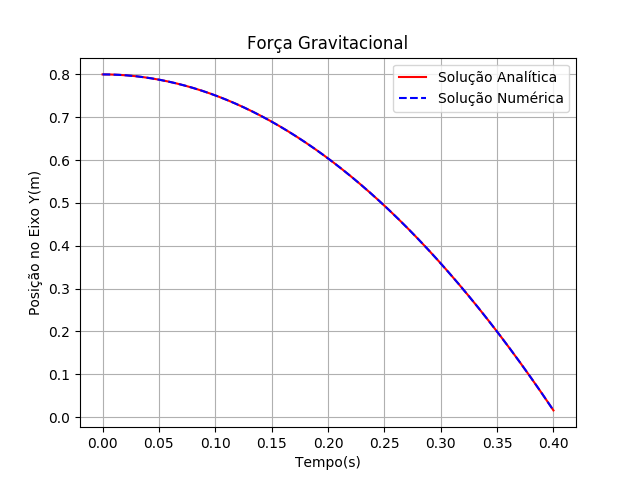
\includegraphics[width=.7\linewidth]{figures/Forces_gravitational_validation.png}
    } {\raggedleft \scriptsize Fonte: Autor.}
    \caption{Comparação de resultado da solução númerica e analítica \ref{grav_sol} do percurso de uma partícula em queda livre.}
    \label{grav_comp}
\end{figure}

%---------------------------------------------------------------------------------------------Segundo Exemplo
\subsection{\textbf{Força de Arrasto}}
\label{sec_drag}
A força de arrasto é a principal fonte de movimentação de uma partícula quando submersa em um fluido em movimento.
A partícula é movimentada pela força de cisalhamento do fluido em transito que exerce atrito sobre sua superfície.
Isto causa um efeito de arrasto, ou carregamento, devido a condição de não escorregamento da superfície da partícula.

Como pode-se analisar pela equação da força \eqref{drag_sol}, quanto maior for a diferença entre os vetores de velocidade da partícula e do fluido maior será a força excercida sobre ela.
E ao se aproximarem da mesma velocidade, a força é reduzida até o ponto de se tornar nula quando a partícula se encontrar com a mesma velocidade do escoamento no mesmo ponto.

Neste caso, a validação é feita para analisar o comportamento da força em relação as propriedades da partícula.

A solução analítica para a posição da partícula sob efeito da força de arrasto no eixo $x$ é:
\begin{equation}
    x(t) = \dfrac{m_p}{c_{d}} (U - v_{x0}) \left(1 - e^{-\frac{c_{d}}{m_p}t}\right) + v_{x0}t + p_{x0}
    \label{drag_sol} 
\end{equation}
define-se $c_{d}$ como:
\begin{equation}
    c_d = 3 \pi \mu_f d_p
    \label{drag_c} 
\end{equation}
onde $m_p$ é a massa da partícula, $\mu_f$ é a viscosidade dinâmica do fluido, $d_p$ é o diâmetro da partícula, $v_{x0}$ é a velocidade e $p_{x0}$ a posição inicial da partícula no eixo $x$.

Foi utilizada a malha padrão com as condições e posição inicial apresentadas na \ref{force_bc}, com velocidade inicial $v_{x0}=0$.
Demonstra-se na \ref{drag_comp} a evolução da posição da partícula no eixo $x$ em função do tempo.
Foi utilizado um campo de velocidades com valor constante de $U=2m/s$.
Pode-se observar que a partícula é acelerada até atingir a velocidade do fluído, como se era esperado.
O erro relativo médio calculado para este caso foi de $3.083e^{-5}\%$ e com desvio padrão de $1.6723e^{-5}\%$.
\begin{figure}[H]
    \centering
    \stackunder{
        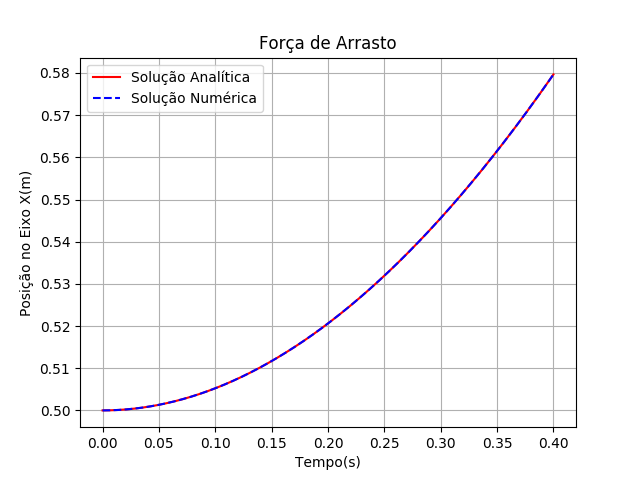
\includegraphics[width=.7\linewidth]{figures/Forces_drag_validation.png}
    } {\raggedleft \scriptsize Fonte: Autor.}
    \caption{Comparação de resultado da solução númerica e analítica \ref{drag_sol} do percurso de uma partícula em movimento de arrasto em um escoamento.}
    \label{drag_comp}
\end{figure}

%---------------------------------------------------------------------------------------------Terceiro Exemplo
\subsection{\textbf{Força de Sustentação}}
\label{sec_lift}
A força de sustentação é a força que permite que a partícula se mantenha elevada quando está sob efeito de um fluido em movimento.
Ela é causada por um efeito de queda de pressão em uma região com maior velocidade, o que gera um gradiente de pressão e enfim a força.

Portanto esta força afeta a partícula somente quando há um gradiente de velocidade ao longo dos contornos da partícula, portanto ela só ocorre quando o campo de velocidades não for constante em volta da partícula.
Esta é a mesma força que possibilita o voo dos aviões, pois os perfis de suas asas geram o gradiente de velocidades necessário.

A força de sustentação possui a seguinte solução analítica para a posição da partícula no eixo $y$ semelhante a força de arrasto \eqref{lift_sol}, porém com constantes diferentes:
\begin{equation}
    y(t) = \dfrac{m_p}{c_l} (0 - v_{y0}) \left(1 - e^{-\frac{c_l}{m_p}t}\right) + v_{y0}t + p_{y0}
    \label{lift_sol} 
\end{equation}
define-se $c_l$ como:
\begin{equation}
    c_l = 1.61 \mu_f d_p \sqrt{{Re}_G}
    \label{lift_c} 
\end{equation}
onde $Re_G$ é o número de Reynolds de cisalhamento\eqref{reg} $\rho_f$ é a densidade do fluido e $\tfrac{dv_x}{dy}$ é a variação da velocidade na partícula sobre o eixo perpendicular ao movimento.

Como é apresentado na \ref{lift_bc}, foi utilizado a mesma malha que nos casos anteriores, porém o campo de velocidade do fluido foi alterado, para que fosse possível observar os efeitos da força de sustentação com mais clareza.
As condições utilizadas são:
\begin{figure}[H]
    \centering
    \stackunder{
        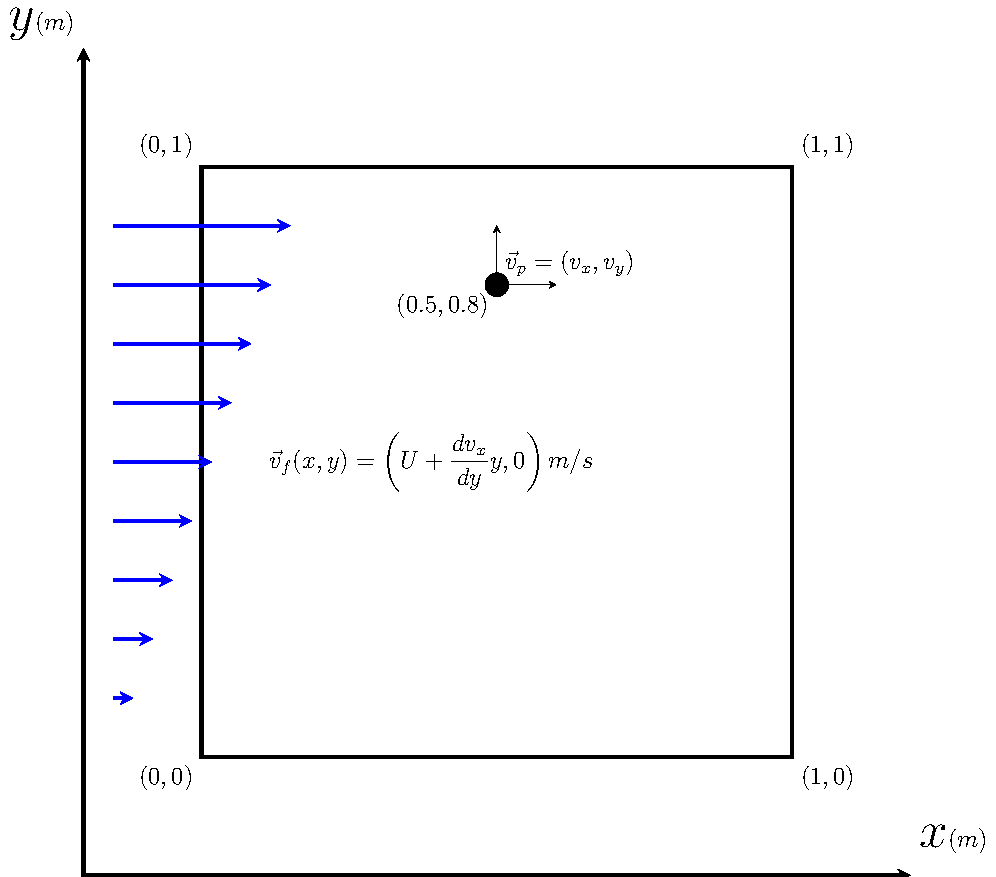
\includegraphics[width=0.7\linewidth]{figures/lift_boundary_conditions.pdf}
    } {\raggedleft \scriptsize Fonte: Autor.}
    \caption{Condições de contorno de uma partícula isolada sob efeito da força de sustentação.}
    \label{lift_bc}
\end{figure}

Demonstra-se na \ref{lift_comp} a evolução da posição da partícula no eixo $x$ em função do tempo.
Foi utilizado um valor base para o campo de velocidades de $U=2m/s$, uma velocidade inicial $v_{y0}=-0.1m/s$, e um gradiente de velocidades no eixo $y$ de $\tfrac{dv_x}{dy}=100m/m.s$ para auxiliar a comparação.
Também foi incluída uma curva que demostra a trajetória da partícula sem o efeito da força de sustentação, para que se possa notar que a partícula é desacelerada e não acompanha esta curva.
O erro relativo médio calculado para este caso foi de $1.9241e^{-6}\%$ e com desvio padrão de $1.1167e^{-6}\%$.
\begin{figure}[H]
    \centering
    \stackunder{
        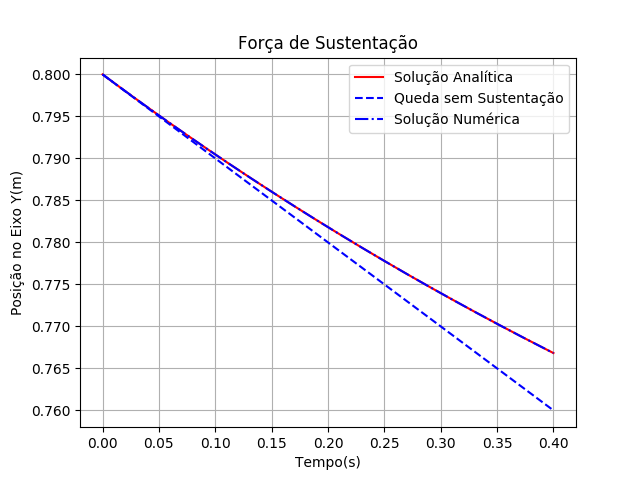
\includegraphics[width=.7\linewidth]{figures/Forces_lift_validation.png}
    } {\raggedleft \scriptsize Fonte: Autor.}
    \caption{Comparação de resultado da solução númerica e analítica \ref{lift_sol} do percurso de uma partícula em movimento de sustentação em um escoamento.}
    \label{lift_comp}
\end{figure}

%---------------------------------------------------------------------------------------------Terceiro Exemplo
\subsection{\textbf{Força de Massa Virtual (\textit{Added Mass})}}
\label{sec_mass}
A força de massa virtual é uma força de reação entre o fluido e a movimentação da partícula durante o escoamento.
O valor dessa força está relacionado a massa de fluido que estaria se deslocando na posição da partícula.

Para encontrar-se a solução analítica da força de massa virtual que pudesse ser observada e comparada com os resultados das simulações, ou seja não sendo nula, foi preciso assumir um campo de velocidades que variasse no tempo.
Para isso, define-se que a aceleração do campo de velocidades do escoamento é constante $\tfrac{d\vec{v}}{dt}=\vec{a}=const$.
Portanto, obtem-se a solução analítica da força de massa virtual para a posição da partícula no eixo $x$.
\begin{equation}
    x(t) = \dfrac{a_x c_m}{2(c_m + m)}t^2 + + v_{x0}t + p_{x0}
    \label{mass_sol} 
\end{equation}
define-se $c_m$ como:
\begin{equation}
    c_m = \dfrac{1}{2} \rho_f V_p
    \label{mass_c} 
\end{equation}
onde $a_x$ é a aceleração, ou variação da velocidade no tempo, do campo de velocidades do fluido no eixo $x$ e $V_p$ é o volume da partícula.

Novamente, foi utilizado a mesma malha e condições dos casos anteriores conforme apresentado na \ref{force_bc}, além disso a condição inicial da componente tangencial da velocidade foi $v_{x0}=0$.
Revela-se na \ref{mass_comp} a evolução da posição da partícula no eixo $x$ em função do tempo.
Foi utilizado um campo de velocidades que varia no tempo com valor constante, como explicado anteriormente, na forma de $U=2m/s+a_x t$, onde $a_x=1m/s^2$.
Pode-se observar que a partícula é acelerada até atingir a velocidade do fluído, como se era esperado.
O erro relativo médio calculado para este caso foi de $6.6574e^{-3}\%$ e com desvio padrão de $1.1362e^{-3}\%$.
\begin{figure}[H]
    \centering
    \stackunder{
        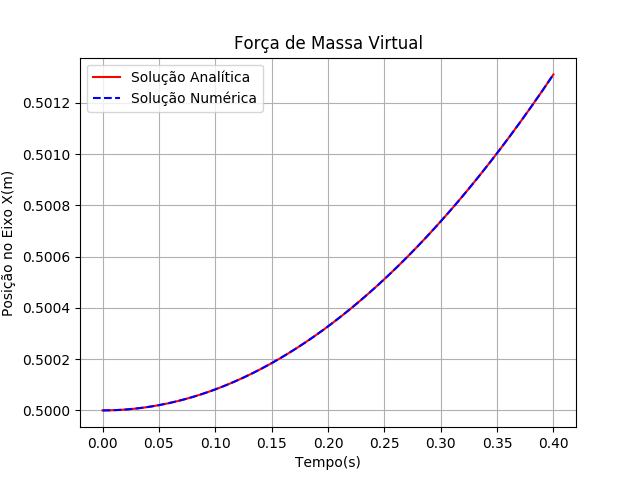
\includegraphics[width=.7\linewidth]{figures/Forces_added_mass_validation.png}
    } {\raggedleft \scriptsize Fonte: Autor.}
    \caption{Comparação de resultado da solução númerica e analítica \ref{mass_sol} do percurso de uma partícula em movimento de aceleração em um escoamento.}
    \label{mass_comp}
\end{figure}